% ==========================================================
% CHƯƠNG 4: THIẾT KẾ VÀ THỰC HIỆN PHẦN MỀM
% ==========================================================

\chapter{Thiết kế và thực hiện phần mềm}
\label{ch:thiet_ke_phan_mem}


\section{Thiết kế và thực hiện phần mềm cập nhật Firmware}
\label{sec:thiet_ke_va_thuc_hien_Bootloader}

\subsection{Yêu cầu thiết kế phần mềm}
\label{sec:yeu_cau_thiet_ke_phan_mem}

Hệ thống hoạt động trong môi trường vệ tinh, vì thế các kỹ sư không thể tiếp cận trực tiếp vào thiết bị để nạp firmware mỗi lần cần cập nhật. Phần mềm cập nhật Firmware được xây dựng nhằm hỗ trợ cập nhật firmware từ xa một cách tin cậy, an toàn và dễ mở rộng. Các yêu cầu thiết kế chính bao gồm:

\textbf{Tổ chức phân lớp rõ ràng:} 
Bootloader được thiết kế theo mô hình phân lớp, bao gồm các thành phần như: Hardware, Driver Flash, Transport (xTP), Command Interface (xCLI) và Bootloader Application Control (xBLD). Cấu trúc này giúp cô lập hoàn toàn logic xử lý dịch vụ khỏi phần cứng ngoại vi, tăng khả năng bảo trì và cho phép dễ dàng tái sử dụng cho các dòng vi điều khiển khác trong tương lai.

\textbf{Đảm bảo tính tin cậy trong truyền dữ liệu:}
Hệ thống bắt buộc phải kiểm soát và ngăn ngừa tuyệt đối hiện tượng sai lệch dữ liệu trong quá trình truyền thông nội bộ giữa các vi xử lý. Do đó, phần mềm cần tích hợp cơ chế phát hiện lỗi vòng CRC và ECC để đảm bảo tính toàn vẹn của dữ liệu firmware được truyền tải.

\textbf{Hỗ trợ cập nhật firmware linh hoạt:}
Chương trình hỗ trợ ghi firmware theo từng khối nhỏ (chunk), cho phép cập nhật từng phần và kiểm tra từng bước để giảm rủi ro lỗi toàn bộ hệ thống. 

\textbf{Quản lý bộ nhớ Flash an toàn:}
Việc ghi, xóa Flash cần đảm bảo không làm ảnh hưởng đến vùng nhớ chứa chương trình cập nhật firmware, đồng thời kiểm soát kích thước và địa chỉ của firmware ứng dụng. 

\textbf{Tự động khởi động ứng dụng:}
Để đảm bảo tính tự động hóa, chương trình sử dụng một bộ đếm thời gian chờ (Idle Timeout). Sau khi khởi động hoặc reset hệ thống, nếu không nhận được lệnh yêu cầu cập nhật từ Host trong một khoảng thời gian quy định, chương trình cập nhật firmware sẽ tự động thực hiện quy trình kiểm tra tính hợp lệ và chuyển quyền thực thi sang ứng dụng chính (User Application).

\subsubsection{Phân tích yêu cầu và phương pháp thực hiện:}
    
    Hệ thống được chia thành hai vùng thực thi riêng biệt:

\textbf{Chương trình cập nhật firmware:} Thành phần quản lý khởi động, đóng vai trò cập nhật firmware cho ứng dụng chính. Chương trình này được thiết kế để hoạt động độc lập, có khả năng nhận lệnh từ Host, ghi dữ liệu vào Flash và kiểm tra tính hợp lệ của firmware trước khi thực thi.

\textbf{Chương trình ứng dụng chính:} Chương trình ứng dụng chính của người dùng, bắt đầu bằng một vùng Header chứa các thông tin của ứng dụng chính như: phiên bản của firmware, phiên bản của hardware, địa chỉ bắt đầu và CRC của ứng dụng chính để chương trình cập nhật phần mềm kiểm tra tính hợp lệ trước khi chuyển sang thực thi.

\begin{figure}[H]
    \centering
    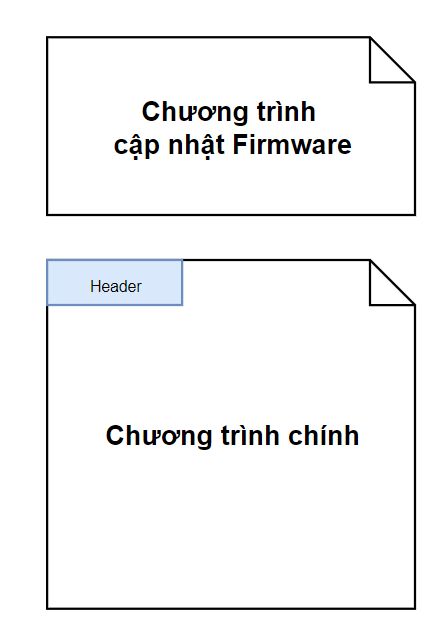
\includegraphics[width=0.5\textwidth]{picture/firmware/Bootloader/flash.png}
    \caption{Tổ chức bộ nhớ Flash}
    \label{fig:to-chuc-bo-nho-flash}
\end{figure}

\begin{itemize}
    \item \textbf{Tổ chức bộ nhớ Flash:}
    \begin{itemize}
        \item Chương trình cập nhật firmware được đặt ở vùng Flash từ 0x00400000 đến 0x0040BFFF (48kB).
        \item Chương trình ứng dụng chính bắt đầu từ 0x0040C000, với Header 512 bytes tại 0x0040C000 và firmware ứng dụng bắt đầu từ 0x0040C200. Kích thước tối đa của chương trình ứng dụng chính khoảng 1.95MB.
        \item Chương trình cập nhật firmware sẽ kiểm tra Header của Chương trình ứng dụng chính để xác định tính hợp lệ trước khi thực thi.
    \end{itemize}

\end{itemize}

Dựa trên các yêu cầu đã đề ra, phương pháp thiết kế Bootloader được tổ chức phân lớp rõ ràng dễ mở rộng và có thể tái sử dụng giao thức xTP cho các ứng dụng khác. Bootloader được chia thành các lớp chính:

\begin{itemize}

    \item \textbf{Driver}: điều khiển phần cứng như Flash, UART. 

    \item \textbf{Transport Layer (xTP)}:
    Cung cấp giao thức truyền dữ liệu dạng frame với các cơ chế: 
    \begin{itemize}
        \item CRC kiểm tra lỗi.
        \item ECC sửa lỗi 1 byte.
        \item Có cơ chế truyền khung truyền lại khi lỗi. 
    \end{itemize}

    \item \textbf{Application Layer (xBLD)}:
    Xử lý các lệnh cho việc cập nhật firmware như ghi, xóa firmware, kiểm tra tính hợp lệ, chuyển sang chương trình ứng dụng. 
    
\end{itemize}

Để đảm bảo tính tin cậy trong truyền dữ liệu, cấu trúc khung truyền xTP được thiết kế như sau:

\begin{figure}[H]
    \centering
    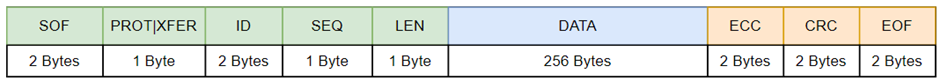
\includegraphics[width=1\textwidth]{picture/firmware/Bootloader/xTP_frame.png}
    \caption{Cấu trúc khung truyền xTP}
    \label{fig:xTP-frame}
\end{figure}

Giao thức xTP được thiết kế như sau:

•   Start of Frame (SOF): 2 byte (0x0C 0xDE) để đánh dấu bắt đầu của một khung tin.

•   PROT|XFER: để thông báo cho phía nhận biết đây là khung truyền cần ACK hay không, sử dụng CRC 16 bit hay CRC 32 bit. 

•   ID Command: 2 byte để xác định lệnh đang được truyền.

•   SEQ: 1 byte để đánh số thứ tự của khung tin, giúp phát hiện mất mát dữ liệu.

•   LEN: 1 byte để xác định độ dài của dữ liệu trong khung tin.

•	ECC (Error Correction Code) để sửa lỗi 1 byte .

•	CRC-16 để phát hiện lỗi dữ liệu.

•   EOF (End of Frame): 2 byte (0xDA 0xED) để đánh dấu kết thúc của một khung tin.

Nhờ đó, quá trình truyền firmware đảm bảo độ tin cậy cao ngay cả khi đường truyền không ổn định.

\begin{figure}[H]
    \centering
    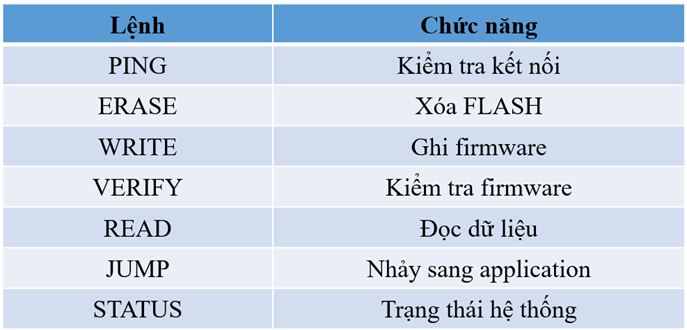
\includegraphics[width=1\textwidth]{picture/firmware/Bootloader/cmd_bootloader.png}
    \caption{Các lệnh điều khiển cho chương trình cập nhật firmware}
    \label{fig:cmd-bootloader}
\end{figure}

\begin{figure}[H]
    \centering
    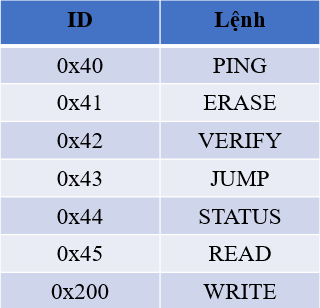
\includegraphics[width=0.7\textwidth]{picture/firmware/Bootloader/cmd-id.png}
    \caption{Các mã ID của lệnh điều khiển}
    \label{fig:cmd-id}
\end{figure}

\subsubsection{Phân tích kịch bản vận hành hệ thống:}


\textbf{Kịch bản 1: Trạng thái chờ và tự động khởi động ứng dụng chính}

Mô tả: Đây là kịch bản mặc định khi thiết bị khởi động mà không có sự can thiệp từ con người.
Mục tiêu: Đảm bảo tính tự động hóa. Nếu sau một khoảng thời gian mà không có lệnh hay không có dữ liệu truyền đến, hệ thống sẽ tự động thực thi ứng dụng chính để đảm bảo thiết bị luôn hoạt động đúng chức năng.


\textbf{Kịch bản 2: Cập nhật phần mềm hệ thống}

Trong kịch bản này, vi điều khiển sẽ tiếp nhận lệnh hoặc dữ liệu firmware cần cập nhật từ một bộ vi xử lý trung gian (MPU).
Mô tả luồng dữ liệu:

\begin{itemize}

\item Dữ liệu đầu vào: Trạm mặt đất truyền file Firmware thông qua các giao thức truyền thông từ xa và tới bộ vi xử lý MPU. MPU sẽ thực hiện các lệnh điều khiển đến MCU để cập nhật firmware thông qua giao thức xTP trên UART.
\item Xử lý tại MCU (xTP Process): đây là giai đoạn thực thi chính của chương trình cập nhật firmware trên vi điều khiển ATSAMV71 để cập nhật chương trình ứng dụng chính.
\item Mục tiêu kỹ thuật:
    \begin{itemize}
        \item Truyền tải tin cậy: Sử dụng giao thức xTP để giải quyết các vấn đề về nhiễu trên đường truyền nội bộ hoặc mất mát dữ liệu. Có cơ chế chia nhỏ file Firmware lớn thành các đoạn dữ liệu có kích thước tối ưu cho bộ nhớ đệm của MCU.
        \item Kiểm soát toàn vẹn của dữ liệu bằng CRC và khi phát hiện lỗi sẽ dùng ECC sửa lỗi nếu lỗi tối đa 1 byte, tăng cường khả năng chịu lỗi cho hệ thống. Dữ liệu chỉ được nạp vào bộ nhớ Flash khi đã vượt qua tất cả các lớp kiểm chứng phần mềm.
    \end{itemize}
        
\end{itemize}



\subsection{Thực hiện phần mềm cập nhật Firmware}
\label{sec:thuc_hien_phan_mem_Bootloader}

\begin{itemize}
    \item \textbf{Lưu đồ giải thuật tổng quát:}
    
    \begin{figure}[H]
        \centering
        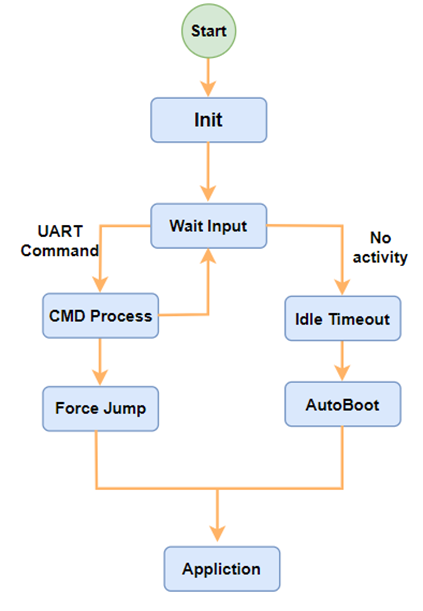
\includegraphics[width=0.7\textwidth]{picture/firmware/Bootloader/Luu_do_tong_quat.png}
        \caption{Lưu đồ giải thuật tổng quát của chương trình cập nhật firmware}
        \label{fig:lưu-đồ-giải-thuật-tổng-quát-của-chương-trình-cập-nhật-firmware}
    \end{figure}

   Sau khi hệ thống được cấp nguồn hoặc reset, chương trình sẽ chuyển sang trạng thái khởi tạo hệ thống cần thiết như UART, giao thức truyền thông xTP để chuẩn bị cho quá trình giao tiếp và cập nhật firmware.

   Sau khi khởi tạo hoàn tất, vi điều khiển sẽ duy trì hoạt động của giao thức truyền thông và chờ các thao tác từ người dùng thông qua UART. Tại đây chương trình liên tục kiểm tra dữ liệu nhận được từ UART để xử lý các lệnh điều khiển, lệnh kiểm tra hệ thống hoặc yêu cầu cập nhật firmware.

   Khi phát hiện dữ liệu đầu vào, hệ thống chuyển sang trạng thái xử lý lệnh. Tùy theo yêu cầu của lệnh nhận được, chương trình sẽ thực hiện xử lí tương ứng như phản hồi việc kiểm tra giao tiếp, yêu cầu nhảy đến chương trình ứng dụng hoặc thực hiện các chức năng hỗ trợ cập nhật firmware. 
   
   Trong trường hợp không có hoạt động truyền nhận dữ liệu hoặc gửi lệnh nào từ phía MPU trong một khoảng thời gian xác định, chương trình tự kiểm tra có tồn ại chương trình chính trong bộ nhớ flash hay không, chướng trình có hợp lệ hay không để tự động chạy ứng dụng chính, giúp hệ thống không bị dừng vô thời hạn trong chế độ cập nhât firmware.
   
   Cuối cùng, khi quá trình nhảy đến chương trình chính hoàn tất, hệ thống bắt đầu thực thi ứng dụng chính.

   \item \textbf{Lưu đồ giải thuật chi tiết:}
   
   Sơ đồ trên mô tả luồng khởi tạo của chương trình cập nhật firmware:

\begin{figure}[H]
    \centering
    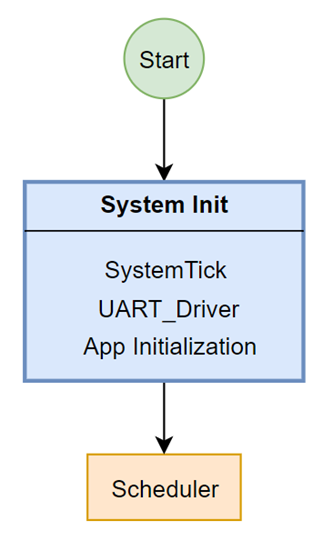
\includegraphics[width=0.4\textwidth]{picture/firmware/Bootloader/init_bootloader.png}
    \caption{Khởi tạo của phan mềm cập nhật firmware}
    \label{fig:khởi-tạo-của-phan-mem-cập-nhật-firmware}
\end{figure}


    Ngay sau khi cấp nguồn hoặc Reset, hệ thống thực hiện các bước chuẩn bị nền tảng tại khối System Init:

    \item \textbf{SystemTick}: Thiết lập bộ đếm thời gian hệ thống, cung cấp cơ sở dữ liệu về thời gian (tick)  và tính toán timeout.
    \item \textbf{UART Driver}: Cấu hình các thông số truyền thông cho cổng giao tiếp UART, thiết lập bộ đệm RX, TX để sẵn sàng nhận lệnh.
    \item \textbf{App Initialization}: Gọi hàm để khởi tạo các ứng dụng con. Tại đây, các ứng dụng cụ thể được thiết lập:

\begin{figure}[H]
    \centering
    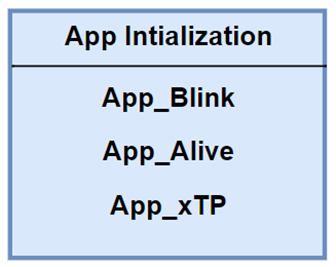
\includegraphics[width=0.4\textwidth]{picture/firmware/Bootloader/init_app.png}
    \caption{Khởi tạo các ứng dụng của phần mềm cập nhật firmware}
    \label{fig:khởi-tạo-cac-ung-dung-cua-phan-mem-cập-nhật-firmware}
\end{figure}

    \item \textbf{App Blink}: Bật tắt LED trạng thái báo hiệu hoạt động của hệ thống.
    \item \textbf{App Alive}: Trong suốt quá trình vận hành, hệ thống sẽ thực hiện reset bộ đếm Watchdog định kỳ nhằm xác nhận phần mềm vẫn đang hoạt động bình thường. Nếu xảy ra hiện tượng treo vi điều khiển hoặc lỗi vòng lặp vô hạn, hành động này sẽ bị bỏ lỡ, Watchdog sẽ bị tràn và tự động khởi động lại hệ thống.
    \item \textbf{App xTP}: Thực hiện việc nhận lệnh, cập nhật firmware và nhảy tới user application. 

    Sau khi hoàn tất khởi tạo, chương trình đi vào vùng scheduler để bắt đầu điều phối quá trình hoạt động của các task. App xTP là ứng dụng chính của chương trình cập nhật firmware, thực hiện 2 nhiệm vụ chính:

\begin{figure}[H]
    \centering
    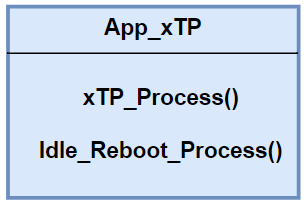
\includegraphics[width=0.4\textwidth]{picture/firmware/Bootloader/app-xTP.png}
    \caption{Các nhiệm vụ của ứng dụng xTP}
    \label{fig:cac-nhiem-vu-cua-ung-dung-xTP}
\end{figure}

    Sơ đồ khối hàm xử lý xTP:

\begin{figure}[H]
    \centering
    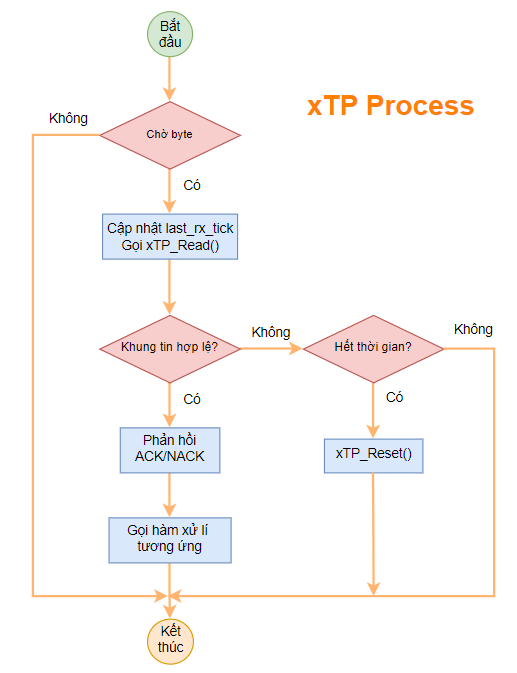
\includegraphics[width=0.8\textwidth]{picture/firmware/Bootloader/block-xTP.png}
    \caption{Sơ đồ khối hàm xử lý xTP}
    \label{fig:so-do-khoi-ham-xTP}
\end{figure}

xTP Process(): Chịu trách nhiệm giải mã luồng dữ liệu thô từ UART theo máy trạng thái của giao thức xTP. Hàm này thực hiện các nhiệm vụ kiểm lỗi và điều phối việc ghi dữ liệu vào Flash khi nhận được các gói tin Firmware hợp lệ. Cụ thể:
\begin{itemize}
    \item Lấy byte dữ liệu: Hệ thống thực hiện quét liên tục. Nếu không có dữ liệu mới, tiến trình sẽ kết thúc ngay lập tức để nhường tài nguyên cho các tác vụ khác.
    \item Cập nhật thời gian thực: Ngay khi nhận được một byte dữ liệu hợp lệ, hệ thống sẽ cập nhật biến last rx tick. Đây là mốc thời gian quan trọng dùng để tính toán Timeout, đảm bảo hệ thống nhận biết được luồng dữ liệu đang được duy trì.
    \item xTP Read(): Byte dữ liệu được đưa vào máy trạng thái (FSM) của giao thức xTP để lắp ghép thành một khung tin (Frame) hoàn chỉnh.
    \item Sau khi xTP Read() xử lý xong một khối dữ liệu, hệ thống tiến hành kiểm tra tính toàn vẹn:
        \begin{itemize}
            \item Nếu Frame hợp lệ: MCU thực hiện gửi phản hồi ACK hoặc NACK (nếu tính toán CRC không khớp và ECC không sửa được lỗi) về cho MPU để xác nhận trạng thái nhận tin, nếu là NACK thì khung tin sẽ được gửi lại. Sau đó, gói tin nhận được sẽ được xử lý bởi hàm đã được định nghĩa ứng với ID lệnh của nó.
            \item Nếu dữ liệu nhận được bị dở dang hoặc sai cấu trúc và không có thêm dữ liệu mới trong một khoảng thời gian nhất định, hệ thống bỏ gói tin và quay về trạng thái chờ ban đầu để sẵn sàng nhận lại gói tin.
        \end{itemize}

\end{itemize}

\begin{figure}[H]
    \centering
    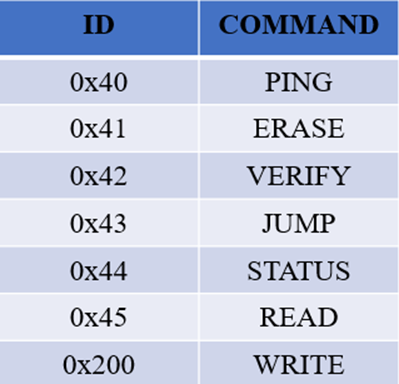
\includegraphics[width=0.5\textwidth]{picture/firmware/Bootloader/command.png}
    \caption{Bảng mã của các lệnh}
    \label{fig:bang-ma-cua-cac-lenh}
\end{figure}


Sơ đồ khối xử lí trạng thái chờ:

\begin{figure}[H]
    \centering
    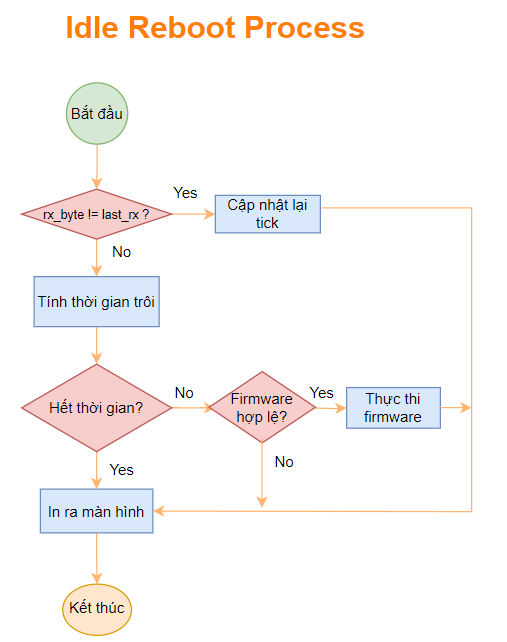
\includegraphics[width=0.8\textwidth]{picture/firmware/Bootloader/block-wait.png}
    \caption{Sơ đồ khối xử lý trạng thái chờ}
    \label{fig:so-do-khoi-xu-ly-trang-thai-cho}
\end{figure}

\begin{itemize}
    \item Idle Reboot Process(): Quản lý thời gian chờ của hệ thống. Nếu không có hoạt động tương tác trong một khoảng thời gian định trước, hàm này sẽ thực hiện kiểm tra tính toàn vẹn của phần mềm cũ và tự động chuyển đổi sang chế độ thực thi ứng dụng chính. Cụ thể:
    \begin{itemize}
        \item Kiểm tra hoạt động nhận tin: Hệ thống kiểm tra xem có dữ liệu nào đang được nhận qua UART hay không? Nếu có hoạt động thì hệ thống ghi lại thời gian nhận được dữ liệu. Nếu không có hoạt động thì hệ thống tiến hành tính toán thời gian trôi qua kể từ lần cuối cùng nhận được dữ liệu.
        \item Nếu quá thời gian chờ thì hệ thống hiểu rằng không có yêu cầu cập nhật Firmware nào đang diễn ra và bắt đầu kiểm tra tính toàn vẹn của ứng dụng đã có trong Flash. Nếu firmware hợp lệ, hệ thống thực hiện lệnh nhảy đến địa chỉ ứng dụng để bắt đầu vận hành thiết bị.
    \end{itemize}
\end{itemize}

\end{itemize}


\section{Thiết kế và thực hiện phần mềm ứng dụng của hệ thống}
\label{sec:thiet_ke_va_thuc_hien_phan_mem_ung_dung}

Để đảm bảo tính linh hoạt, dễ bảo trì và khả năng mở rộng, firmware của hệ thống được thiết kế theo mô hình phân lớp. Cấu trúc này giúp tách biệt giữa logic ứng dụng và các thao tác điều khiển phần cứng cấp thấp.

\begin{figure}[H]
    \centering
    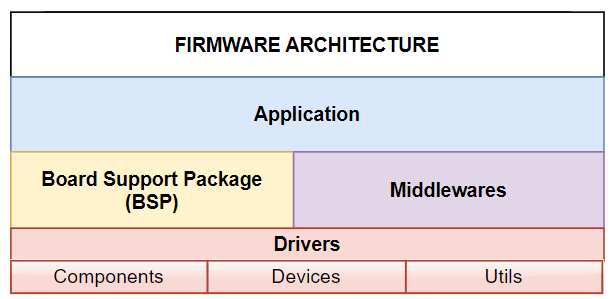
\includegraphics[width=0.9\textwidth]{picture/firmware/kien_truc.png}
    \caption{Kiến trúc phân lớp của hệ thống}
    \label{fig:kien-truc-phan-lop-cua-he-thong}
\end{figure}


Quá trình thiết kế firmware cần tuân thủ các tiêu chí kỹ thuật khắt khe nhằm đảm bảo hệ thống vận hành ổn định trong môi trường thực tế:
\begin{itemize}

\item \textbf{Tổ chức phân lớp rõ ràng:}Tách biệt hoàn toàn giữa Driver, Board Support Package, Middleware và Application. Điều này cho phép thay đổi linh kiện phần cứng mà không cần viết lại toàn bộ mã nguồn ứng dụng.
\item \textbf{Đáp ứng tính thời gian thực (Real-time):} Sử dụng cơ chế lập trình hướng sự kiện kết hợp với FreeRTOS để xử lý nhiều tác vụ như điều khiển nhiệt độ, thực hiện thí nghiệm, lưu trữ mẫu và nhận lệnh từ MPU.
\item \textbf{Quản lý đa ngoại vi phức tạp:} Firmware phải điều phối nhịp nhàng việc giao tiếp cùng lúc với nhiều mô-đun (Laser, Photo, TEC, HEATER, PRAM).
\item \textbf{Khả năng mở rộng và tái sử dụng:} Thiết kế theo dạng mô-đun hóa giúp việc nâng cấp tính năng hoặc tích hợp thêm cảm biến mới trở nên đơn giản.

\end{itemize}

Kiến trúc firmware thực hiện được chia thành các lớp chính như sau:

\begin{figure}[H]
    \centering
    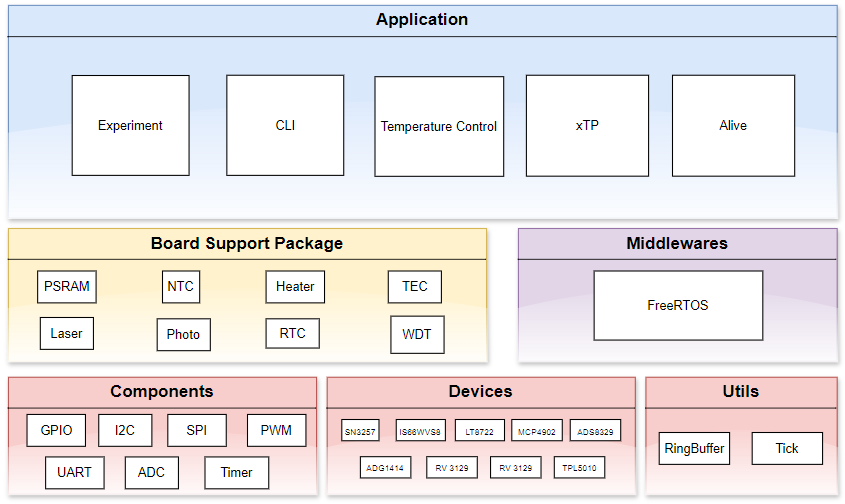
\includegraphics[width=0.9\textwidth]{picture/firmware/tp_kien_truc.png}
    \caption{Các thành phần của phân lớp của hệ thống}
    \label{fig:cac-thanh-phan-cua-phan-lop-cua-he-thong}
\end{figure}

\begin{itemize}
    \item \textbf{Application}: Chứa logic điều khiển chính của hệ thống bao gồm quản lý tiến trình thí nghiệm (Experiment), xử lý lệnh người dùng (CLI), điều khiển nhiệt độ (Temperature Control), và đảm bảo hoạt động của hệ thống (Alive).
    \item \textbf{Board Support Package (BSP)}: Cung cấp các hàm để tương tác với các khối chức năng cụ thể trên board mạch như Laser, Heater, TEC, NTC, RTC và Watchdog Timer (WDT).
    \item \textbf{Middleware}: Thành phần trung gian cung cấp hệ điều hành thời gian thực FreeRTOS để quản lý đa nhiệm.
    \item \textbf{Drivers \& Components}: Bao gồm các trình điều khiển cho các chuẩn giao tiếp vật lý (GPIO, I2C, SPI, UART, ADC) và các linh kiện điện tử cụ thể (như MCP4902, ADS8329, RV 3129).
    \item \textbf{Utils}: Các công cụ hỗ trợ như quản lý bộ đệm vòng (RingBuffer) và bộ đếm thời gian (Tick).

\end{itemize}

\subsection{Thiết kế và thực hiện phần mềm thí nghiệm}
\label{sec:yeu_cau_thiet_ke_phan_mem_thi_nghiem}

\subsubsection{Phân tích yêu cầu và phương pháp thực hiện:}

Hệ thống được xây dựng nhằm phục vụ quá trình điều khiển bật, tắt và điều chỉnh cường độ laser, đồng thời thu thập và lưu trữ dữ liệu ADC, đọc về tốc độ cao từ các photo diode theo tần số mong muốn. Vì vậy, mục tiêu thiết kế:

    \begin{itemize}
        \item Bật tắt và duy trì dòng điện chính xác cho laser.
        \item Duy trì lấy mẫu liên tục theo tần số mong muốn trong những khoảng thời gian nhất định theo thời gian thực.
        \item Tránh mất dữ liệu khi tốc độ lấy mẫu cao.
        \item Đồng thời vẫn ghi được dữ liệu xuống bộ nhớ ngoài.
    \end{itemize}
    Vì vậy, hệ thống được tổ chức theo hướng xử lý bất đồng bộ (asynchronous processing), trong đó các thành phần lấy mẫu và lưu trữ hoạt động độc lập thông qua Queue.
    
    \begin{itemize}

    \item Phân tích kiến trúc hệ thống:
    \begin{itemize}
        \item \textbf{Photo Sampling}: Thu thập dữ liệu ADC và đẩy vào Queue.
        \item \textbf{Laser Control}: Bật tắt laser và điều khiển dòng cho laser thông qua giao tiếp SPI.
        \item \textbf{Store to PRAM}: Lấy dữ liệu từ Queue lưu vào PRAM.
    \end{itemize}

    \item Phân tích kịch bản vận hành hệ thống:
    \begin{itemize}
        \item \textbf{Khởi động hệ thống}: Sau khi khởi động, hệ thống chờ nhận lệnh bắt đầu thí nghiệm.
        \item \textbf{Bắt đầu thí nghiệm}: Khi lệnh được nhận, tác vụ điều khiển sẽ bật laser theo thời gian yêu cầu, kích hoạt thời gian lấy mẫu, bắt đầu thu dữ liệu ADC và ghi dữ liệu vào  vào PSRAM.
    \end{itemize}

\end{itemize}


\subsubsection{Thực hiện phần mềm thí nghiệm:}

\begin{itemize}
    
    \item \textbf{Lưu đồ giải thuật tổng quát:}

    \begin{figure}[H]
        \centering
        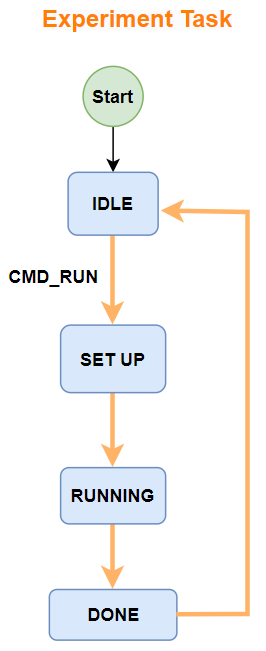
\includegraphics[width=0.3\textwidth]{picture/firmware/Experiment/block-tong-quat.png}
        \caption{Lưu đồ giải thuật tổng quát của phần mềm thí nghiệm}
        \label{fig:lưu-đồ-giải-thuật-tổng-quát-của-phần-mềm-thí-nghiệm}
    \end{figure}

Tiến trình chính của thí nghiệm được phân chia thành 4 giai đoạn:

    \begin{itemize}
        \item \textbf{IDLE:} Trạng thái chờ lệnh. Hệ thống sẽ duy trì ở trạng thái này cho đến khi nhận được lệnh EXP CMD RUN
        \item \textbf{SET UP:} Thực hiện cấu hình các tham số vật lý cho thí nghiệm như: thời gian lấy mẫu, tốc độ lấy mẫu, cường độ Laser, khởi tạo kênh đo và bật switch giao tiếp giữa MCU và PSRAM.
        \item \textbf{RUNNING:} MCU sẽ điều khiển bật, tắt các kênh Laser và Photo tương ứng, đồng thời kích hoạt quá trình thu thập dữ liệu tự động. Việc thu thập mẫu ADC được thực hiện ở 3 pha đo: truớc khi bật laser (pre phase), trong khi laser đang bật (main phase) và sau khi tắt laser (after phase). 

        \begin{figure}[H]
            \centering
            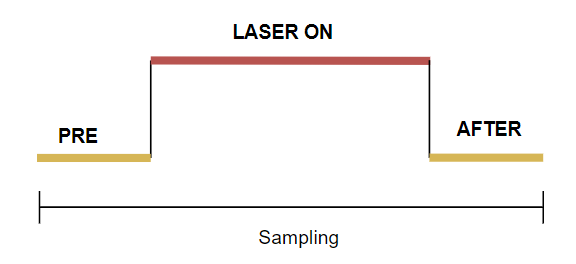
\includegraphics[width=0.9\textwidth]{picture/firmware/Experiment/phase-laser.png}
            \caption{Các pha thu thập dữ liệu trong quá trình thí nghiệm}
            \label{fig:lược-đo-tuan-tu}
        \end{figure}

        \item \textbf{DONE:} Kết thúc quá trình đo, giải phóng tài nguyên và quay trở lại trạng thái IDLE để sẵn sàng cho chu kỳ tiếp theo.
    \end{itemize}

Mô tả chi tiết quá trình thu thập dữ liệu theo tần số mong muốn:

    \begin{figure}[H]
        \centering
        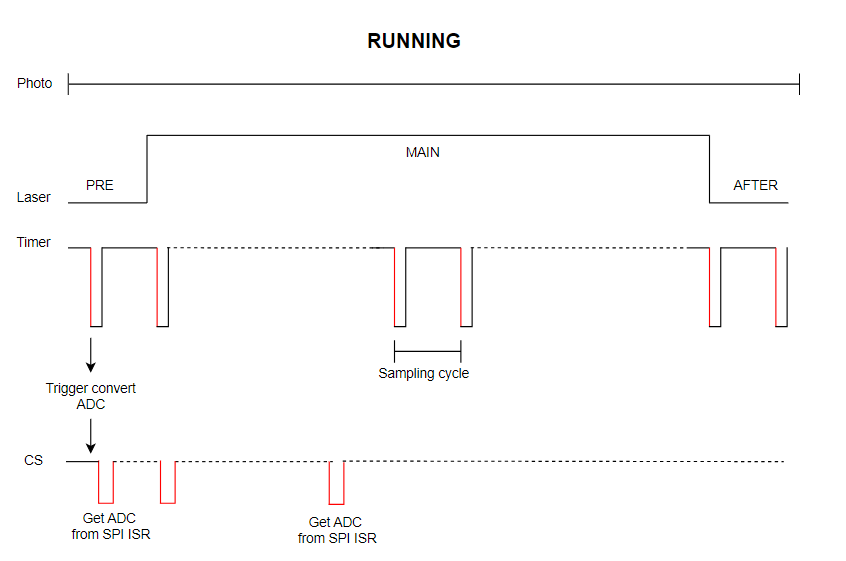
\includegraphics[width=0.9\textwidth]{picture/firmware/Experiment/chi-tiet-lay-mau.png}
        \caption{Mô tả chi tiết quá trình thu thập dữ liệu}
        \label{fig:chi-tiet-lay-mau}
    \end{figure}

    \begin{itemize}
        \item Đầu tiên, tác vụ thí nghiệm thực hiện cấu hình các tham số và kích hoạt bộ định thời và bật Photo cần đo.
        \item Bộ định thời được cấu hình theo đúng tần số lấy mẫu mong muốn của lệnh gửi vào để tự động kích hoạt chân chuyển đổi ADC của IC ADS8329, sau đó kéo chân CS của IC xuống để giao tiếp SPI.
        \item Trình phục vụ ngắt SPI tiếp nhận giá trị ADC được gửi về, lưu trữ vào bộ đệm và kéo chân CS lên. Khi bộ đệm đầy, thực hiện gửi buffer vào hàng đợi. Quá trình lấy mẫu được thực hiện ở cả 3 pha trước khi bật laser (pre phase), trong khi laser đang bật (main phase) và sau khi tắt laser (after phase).

    \end{itemize}

    \item \textbf{Lưu đồ giải thuật chi tiết:}
    
    Sơ đồ trạng thái RUNNING trong thí nghiệm:

    \begin{figure}[H]
        \centering
        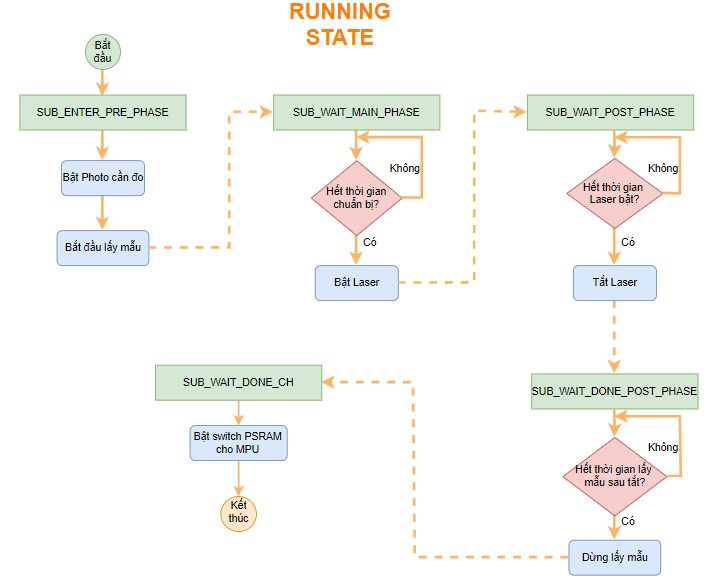
\includegraphics[width=1\textwidth]{picture/firmware/Experiment/running-state.png}
        \caption{Sơ đồ trạng thái RUNNING}
        \label{fig:running-state}
    \end{figure}
    
    Quá trình xử lý cho mỗi kênh đơn lẻ được chia thành 4 trạng thái logic kế tiếp nhau:

    \begin{itemize}
        \item \textbf{SUB ENTER PRE PHASE}: Hệ thống thực hiện chuyển mạch sang kênh photo tương ứng để bắt đầu lấy mẫu từ ADC. 
        \item \textbf{SUB WAIT MAIN PHASE}: Hệ thống kiểm tra thời gian trôi qua so với giá trị predelay. Nếu đủ thời gian thì thực hiện nạp mã DAC cho IC MCP4902 để điều khiển cường độ sáng và kích hoạt Laser, sau đó chuyển sang giai đoạn đo chính.
        \item \textbf{SUB WAIT POST PHASE}: Dữ liệu được thu thập liên tục trong khi Laser đang bật. Khi thời gian đạt ngưỡng thòi gian lấy mẫu, hệ thống tắt Laser và đưa giá trị DAC về 0.
        \item \textbf{SUB WAIT DONE POST PHASE}: Hệ thống duy trì việc lấy mẫu thêm một khoảng thời gian để ghi nhận sự phản ứng của photo sau khi ngắt nguồn sáng. 
        \item \textbf{SUB WAIT DONE}: Hệ thống dừng bộ định thời kích hoạt lấy mẫu, bật switch giao tiếp giữa MPU và PSRAM và bật chân GPIO để báo hiệu hoàn thành đo cho MPU.
    \end{itemize}

    Sơ đồ xử lý ngắt lấy mẫu ADC:
        \begin{figure}[H]
        \centering
        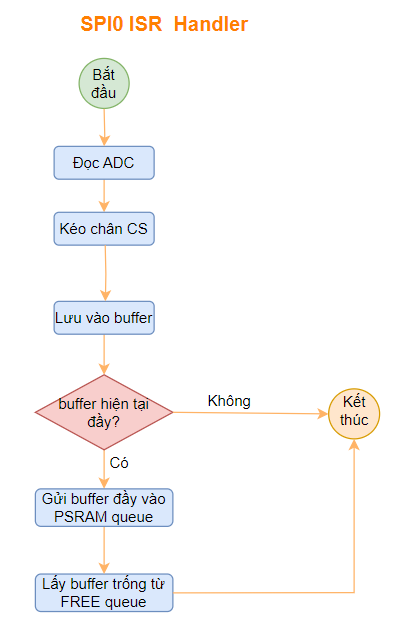
\includegraphics[width=0.7\textwidth]{picture/firmware/Experiment/spi_isr.png}
        \caption{Sơ đồ xử lý ngắt lấy mẫu ADC}
        \label{fig:spi_isr}
    \end{figure}

    \begin{itemize}
        \item Ngay khi ngắt SPI được kích hoạt, hệ thống thực hiện đọc dữ liệu ADC được gửi về từ IC ADS8329 và kéo chân CS lên để kết thúc giao tiếp SPI.
        \item Để đảm bảo việc lấy mẫu liên tục ở tần số cao mà không bị mất mát dữ liệu, giải thuật sử dụng cơ chế hoán đổi bộ đệm tự động ngay trong ISR:
        \begin{itemize}
            \item Kiểm tra độ đầy: sau mỗi lần ghi dữ liệu, chỉ số buf idx được cập nhật. Hệ thống kiểm tra xem bộ đệm đầy chưa. Nếu bộ đệm hiện tại đã đầy, ISR thực hiện hai thao tác đồng thời:
            \begin{enumerate}
                \item Đẩy con trỏ bộ đệm vừa đầy vào PSRAM queue để tác vụ lưu trữ PSRAM xử lý.
                \item Lấy một con trỏ bộ đệm trống từ FREE queue để gán làm current buf mới và reset chỉ số về 0.
            \end{enumerate}
        \end{itemize}
    \end{itemize}

    Sơ đồ khối tác vụ PSRAM:
    \begin{figure}[H]
        \centering
        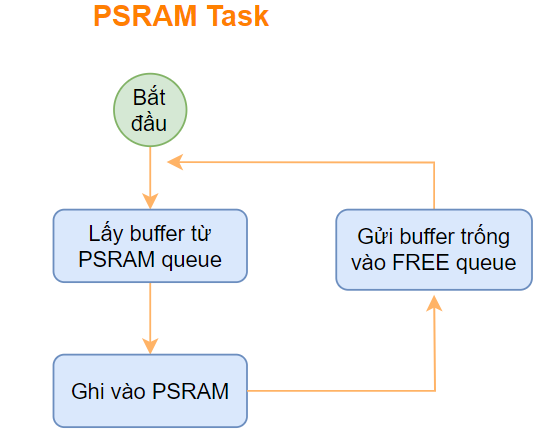
\includegraphics[width=0.6\textwidth]{picture/firmware/Experiment/psram.png}
        \caption{Sơ đồ khối tác vụ PSRAM}
        \label{fig:psram-task}
    \end{figure}

    Tác vụ PSRAM nhận dữ liệu từ hàng đợi, thực hiện lưu trữ vào trong PSRAM và sau đó đẩy con trỏ bộ đệm đã lưu xong vào FREE queue.

\end{itemize}


\subsection{Thiết kế và thực hiện phần mềm giám sát nhiệt độ}
\label{sec:yeu_cau_thiet_ke_phan_mem_giam_sat_nhiet_do}


\subsubsection{Phân tích yêu cầu và phương pháp thực hiện}

Hệ thống được thiết kế để điều khiển chính xác nhiệt độ theo kịch bản có sẵn được cấu hình trong 1 Profile, phục vụ cho các quy trình thí nghiệm khác nhau. Profile này là 1 struct với các trường cung cấp thông tin về trạng thái hoạt động của 1 profile, 2 NTC được chọn để giám sát nhiệt độ, TEC và HEATER được chọn để điều khiển nhiệt độ, các giai đoạn tăng nhiệt, giảm nhiệt và giữ nhiệt với các thông số cụ thể về nhiệt độ mục tiêu, thời gian thực hiện và dải sai số cho phép. Và hệ thống có thể vận hành 8 Profile độc lập và các profile được cấu hình bằng lệnh.

\paragraph{Mục tiêu thiết kế}
\begin{itemize}
    \item \textbf{Điều khiển chính xác:} Duy trì nhiệt độ bám sát giá trị \textit{setpoint} với sai số tối thiểu thông qua thuật toán PID.
    
    \item \textbf{Quản lý quỹ đạo (Profile):} Thực thi các giai đoạn tăng nhiệt, giảm nhiệt và giữ nhiệt theo cấu hình định trước trong Profile.
\end{itemize}

\paragraph{a. Các chức năng của hệ thống}
\begin{itemize}
    \item Thu thập dữ liệu ADC từ cảm biến NTC.
    
    \item Máy trạng thái điều phối các giai đoạn:
    \texttt{Disable}, \texttt{Preheat}, \texttt{Heating/Cooling}, \texttt{Soak} và \texttt{Error}.
    
    \item Xuất tín hiệu PWM để điều khiển công suất thiết bị điều khiển nhiệt độ (\textit{Heater}/TEC) dựa trên kết quả tính toán của bộ PID.
\end{itemize}

\paragraph{b. Phân tích kịch bản vận hành hệ thống}

\begin{itemize}

    \item \textbf{Gia nhiệt sơ bộ (Preheat)}
    
    \begin{itemize}
        \item \textbf{Mô tả:} Xảy ra ngay khi nhận lệnh \texttt{CMD\_AUTO}. Hệ thống đưa nhiệt độ về điểm bắt đầu của quy trình.
        
        \item \textbf{Mục tiêu:} Đảm bảo hệ thống đạt trạng thái ổn định trước khi bắt đầu đếm thời gian. 
        
        Tùy vào nhiệt độ thực tế, hệ thống tự động rẽ nhánh sang:
        \texttt{PREHEAT\_HEAT} hoặc \texttt{PREHEAT\_COOL}.
    \end{itemize}

    \item \textbf{Thực thi quỹ đạo}
    
    \begin{itemize}
        \item \textbf{Mô tả:} Đây là lúc hệ thống bắt đầu điều khiển nhiệt độ theo kịch bản đã cấu hình trong Profile sau khi nhận được lệnh kích hoạt \texttt{CMD\_START}.
        
        \item \textbf{Mục tiêu:}
        
        \begin{itemize}
            \item \textbf{Giai đoạn gia nhiệt hoặc giảm nhiệt:} Hệ thống dựa trên nhiệt độ mong muốn và đạt được trong bao lâu để tính toán và điều khiển \textit{setpoint} theo thời gian thực đảm bảo nhiệt độ thay đổi mượt mà.
            
            \item \textbf{Giai đoạn Soak:} Kích hoạt bộ đếm thời gian (\texttt{sw\_timer}) để duy trì nhiệt độ thực tế nằm trong dải sai số cho phép (\texttt{SOAK\_TEMP\_BAND\_C}) trong thời gian quy định. Sau khi hết thời gian, hệ thống tự động chuyển sang bước tiếp theo trong Profile.
            
        \end{itemize}
    \end{itemize}

\end{itemize}

\subsubsection{Thực hiện phần mềm giám sát nhiệt độ:}

\begin{itemize}

    
    \item \textbf{Lưu đồ giải thuật tổng quát:}
    
    \begin{figure}[H]
        \centering
        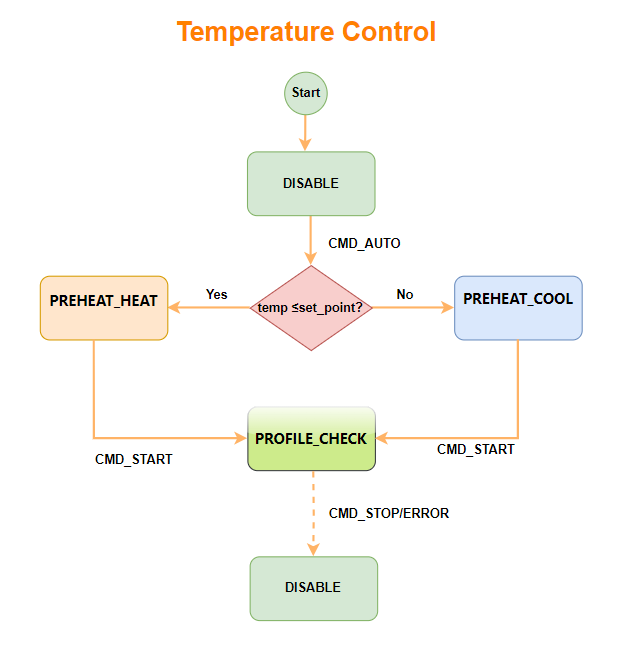
\includegraphics[width=1\textwidth]{picture/firmware/Temperature_Control/temperature-task.png}
        \caption{Lưu đồ giải thuật tổng quát của phần mềm điều khiển nhiệt độ}
        \label{fig:lưu-đồ-giải-thuật-tổng-quát-của-phần-mềm-điều-khiển-nhiệt-độ}
    \end{figure}

    \begin{figure}[H]
        \centering
        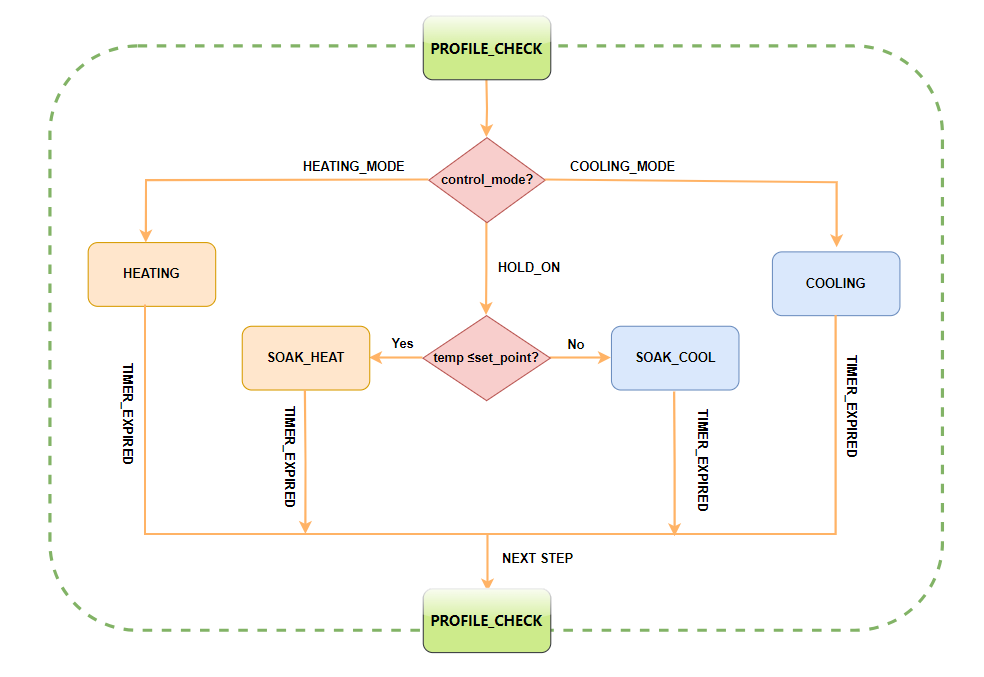
\includegraphics[width=1\textwidth]{picture/firmware/Temperature_Control/state-machine-profile.png}
        \caption{Lưu đồ giải thuật tổng quát của phần mềm điều khiển nhiệt độ}
        \label{fig:lưu-đồ-giải-thuật-tổng-quát-của-phần-mềm-điều-khiển-nhiệt-độ}
    \end{figure}

    \paragraph{Nguyên lý vận hành hệ thống:}

Hệ thống vận hành tuần tự qua các giai đoạn điều khiển nhiệt độ khác nhau như sau:

\begin{itemize}

    \item \textbf{DISABLE:} 
    
    Đây là trạng thái nghỉ của hệ thống. Toàn bộ đầu ra công suất như Heater và TEC được đưa về mức 0\%.
    
    Hệ thống chờ nhận lệnh \texttt{CMD\_AUTO} để bắt đầu nạp dữ liệu \textit{Profile} và chuyển sang giai đoạn \texttt{PREHEAT}.

    \item \textbf{PREHEAT:}
    
    Hệ thống tự động so sánh nhiệt độ hiện tại với giá trị đặt (\textit{setpoint}):
    
    \begin{itemize}
        \item Nếu nhiệt độ thấp hơn \textit{setpoint}: chuyển sang trạng thái \texttt{PREHEAT\_HEAT} để kích hoạt Heater.
        
        \item Nếu nhiệt độ cao hơn \textit{setpoint}: chuyển sang trạng thái \texttt{PREHEAT\_COOL} để kích hoạt TEC.
    \end{itemize}
    
    Mục tiêu của giai đoạn này là đưa hệ thống vào vùng ổn định nhiệt trước khi thực hiện các bước tiếp theo trong quy trình.

    \item \textbf{PROFILE\_CHECK:}
    
    Hệ thống tăng chỉ số \texttt{current\_step} và kiểm tra \texttt{control\_mode} của bước kế tiếp để quyết định chuyển sang các trạng thái:
    
    \begin{itemize}
        \item \texttt{HEATING}
        \item \texttt{COOLING}
        \item \texttt{SOAK}
    \end{itemize}

    \item \textbf{HEATING / COOLING:}
    
    Hệ thống sử dụng thuật toán PID để điều khiển quá trình thay đổi nhiệt độ theo thời gian bằng cách chia nhỏ quỹ đạo nhiệt độ thành các điểm \textit{setpoint} trung gian để sử dụng PID điều khiển công suất đầu ra của Heater hoặc TEC. Quá trình điều khiển đảm bảo nhiệt độ thay đổi mượt, hạn chế hiện tượng quá điều chỉnh (overshoot) và sốc nhiệt. Sau khi hết thời gian quy định, hệ thống quay lại trạng thái \texttt{PROFILE\_CHECK} để thực hiện bước tiếp theo nếu còn tồn tại trong Profile.


    \item \textbf{SOAK (Ngâm nhiệt):}
    
    Hệ thống duy trì nhiệt độ ổn định tại giá trị \textit{setpoint} trong một khoảng thời gian xác định trước. Sau khi hết thời gian quy định, hệ thống quay lại trạng thái \texttt{PROFILE\_CHECK} để thực hiện bước tiếp theo nếu còn tồn tại trong Profile.

    \item \textbf{Dừng hệ thống:}
    
    Hệ thống sẽ dừng hoạt động trong các trường hợp sau:
    
    \begin{itemize}
        \item Nhận lệnh \texttt{CMD\_STOP} từ người vận hành.
        
        \item Phát hiện lỗi trong quá trình hoạt động.
    \end{itemize}

\end{itemize}


    \item \textbf{Lưu đồ giải thuật chi tiết:}
    
    \begin{figure}[H]
        \centering
        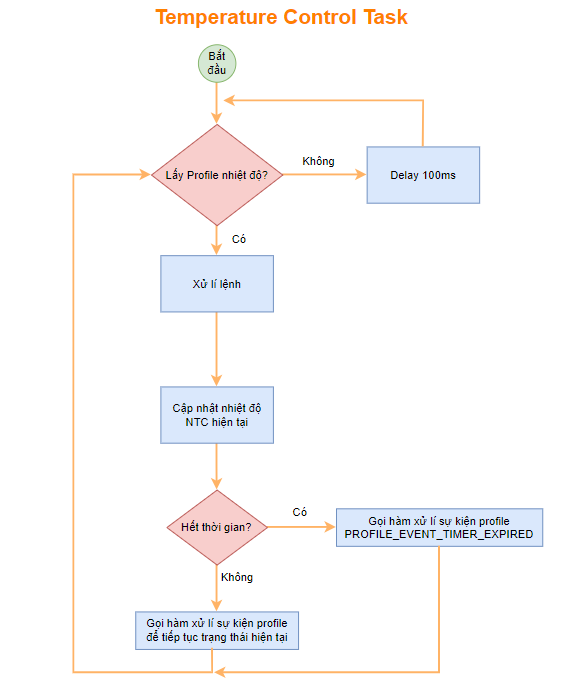
\includegraphics[width=1\textwidth]{picture/firmware/Temperature_Control/task-control.png}
        \caption{Lưu đồ giải thuật của tác vụ điều khiển nhiệt độ}
        \label{fig:lưu-đồ-giải-thuật-cua-tác-vụ-điều-khiển-nhiệt-độ}
    \end{figure}
    
    \paragraph{Chu trình xử lý chính của hệ thống}

\begin{itemize}

    \item \textbf{Kiểm tra trạng thái Profile}
    
    Khi bắt đầu mỗi chu kỳ xử lý, hệ thống sẽ lấy \textit{Profile} để kiểm tra xem có \textit{Profile} nhiệt độ đang hoạt động và cần được xử lý hay không.
    
    \begin{itemize}
        \item Nếu không tồn tại \textit{Profile} hoạt động, tác vụ sẽ thực hiện lệnh \texttt{Delay 100\,ms} trước khi quay lại vòng lặp kiểm tra ban đầu.
        
        \item Nếu tồn tại \textit{Profile} đang hoạt động, hệ thống tiếp tục đi sâu vào các bước xử lý logic tiếp theo.
    \end{itemize}

    \item \textbf{Xử lý lệnh điều khiển}
    
    Hệ thống tiếp nhận và thực thi các lệnh điều khiển, bao gồm:
    
    \begin{itemize}
        \item Bật trạng thái hoạt động của Profile (\texttt{AUTO})
        \item Bắt đầu điều khiển nhiệt độ theo Profile (\texttt{START})
        \item Dừng hoạt động của Profile (\texttt{STOP})
        
    \end{itemize}
    
    Các lệnh này sẽ tác động trực tiếp đến trạng thái hiện tại của máy trạng thái điều khiển nhiệt độ.

    \item \textbf{Cập nhật dữ liệu hệ thống}
    
    Hệ thống thực hiện:
    
    \begin{itemize}
        \item Cập nhật Profile cho hệ thống điều khiển.
        \item Đọc dữ liệu nhiệt độ từ cảm biến NTC thông qua ADC.              
    \end{itemize}

    \item \textbf{Kiểm tra điều kiện thời gian}
    
    Hệ thống kiểm tra thời gian của bước hiện tại:
    
    \begin{itemize}
        \item Nếu hết thời gian quy định:
        
        Kích hoạt sự kiện:
        \texttt{PROFILE\_EVENT\_TIMER\_EXPIRED}.
        
        \item Nếu chưa hết thời gian:
        
        Hệ thống duy trì trạng thái hiện tại của hệ thống.
    \end{itemize}

    \item \textbf{Lặp chu trình điều khiển}
    
    Sau khi xử lý sự kiện, luồng điều khiển quay trở lại bước kiểm tra \textit{Profile} để bắt đầu một chu kỳ quét mới.
    
    Cơ chế này đảm bảo hệ thống hoạt động liên tục, đáp ứng thời gian thực và duy trì tính ổn định của quá trình điều khiển nhiệt độ.

\end{itemize}

    \begin{figure}[H]
        \centering
        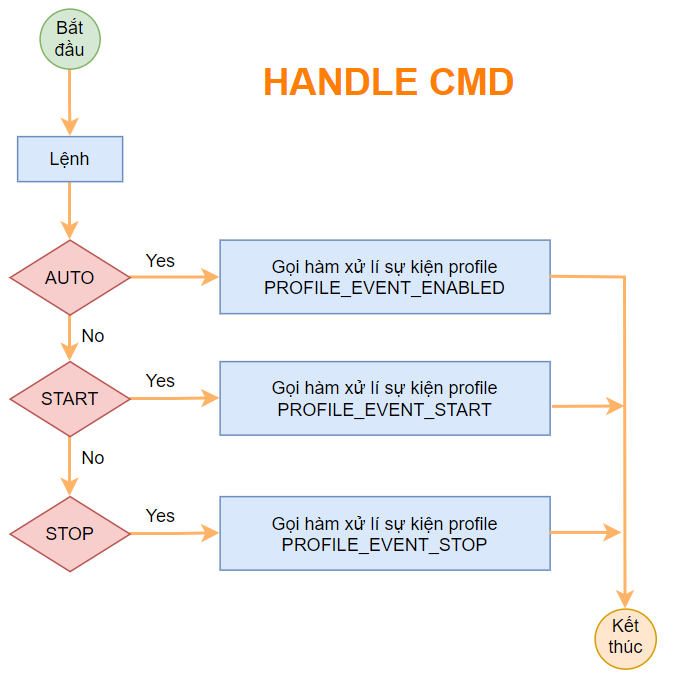
\includegraphics[width=0.7\textwidth]{picture/firmware/Temperature_Control/handle-cmd.png}
        \caption{Lưu đồ giải thuật xử lý lệnh điều khiển của phần mềm giám sát nhiệt độ}
        \label{fig:lưu-đồ-giải-thuật-xử-lý-lệnh-điều-khiển-của-phần-mềm-giám-sát-nhiệt-độ}
    \end{figure}

Khi một lệnh điều khiển của 1 Profile được gửi đến, hệ thống sẽ thực hiện phân loại và kích hoạt các sự kiện tương ứng để điều phối hoạt động của máy trạng thái.

\begin{itemize}

    \item \textbf{Lệnh AUTO}
    
    Khi nhận lệnh \texttt{AUTO}, hệ thống kích hoạt sự kiện:
    
    \begin{center}
        \texttt{PROFILE\_EVENT\_ENABLED}
    \end{center}
    
    Sự kiện này đưa hệ thống từ trạng thái nghỉ (\texttt{DISABLE}) sang giai đoạn chuẩn bị (\texttt{PREHEAT}) nhằm thiết lập điều kiện nhiệt độ ban đầu cho quá trình vận hành.

    \item \textbf{Lệnh START}
    
    Khi nhận lệnh \texttt{START}, hệ thống kích hoạt sự kiện:
    
    \begin{center}
        \texttt{PROFILE\_EVENT\_START}
    \end{center}
    
    Sự kiện này cho phép hệ thống bắt đầu thực thi các bước trong \textit{Profile} sau khi quá trình ổn định nhiệt độ sơ bộ hoàn tất.

    \item \textbf{Lệnh STOP}
    
    Khi nhận lệnh \texttt{STOP}, hệ thống kích hoạt sự kiện:
    
    \begin{center}
        \texttt{PROFILE\_EVENT\_STOP}
    \end{center}
    
    Hệ thống sẽ lập tức dừng toàn bộ hoạt động điều khiển, ngắt các đầu ra công suất và quay trở về trạng thái an toàn.

\end{itemize}

Sơ đồ khối xử lý sự kiện (Profile Handle Event):

\begin{figure}[H]
    \centering
    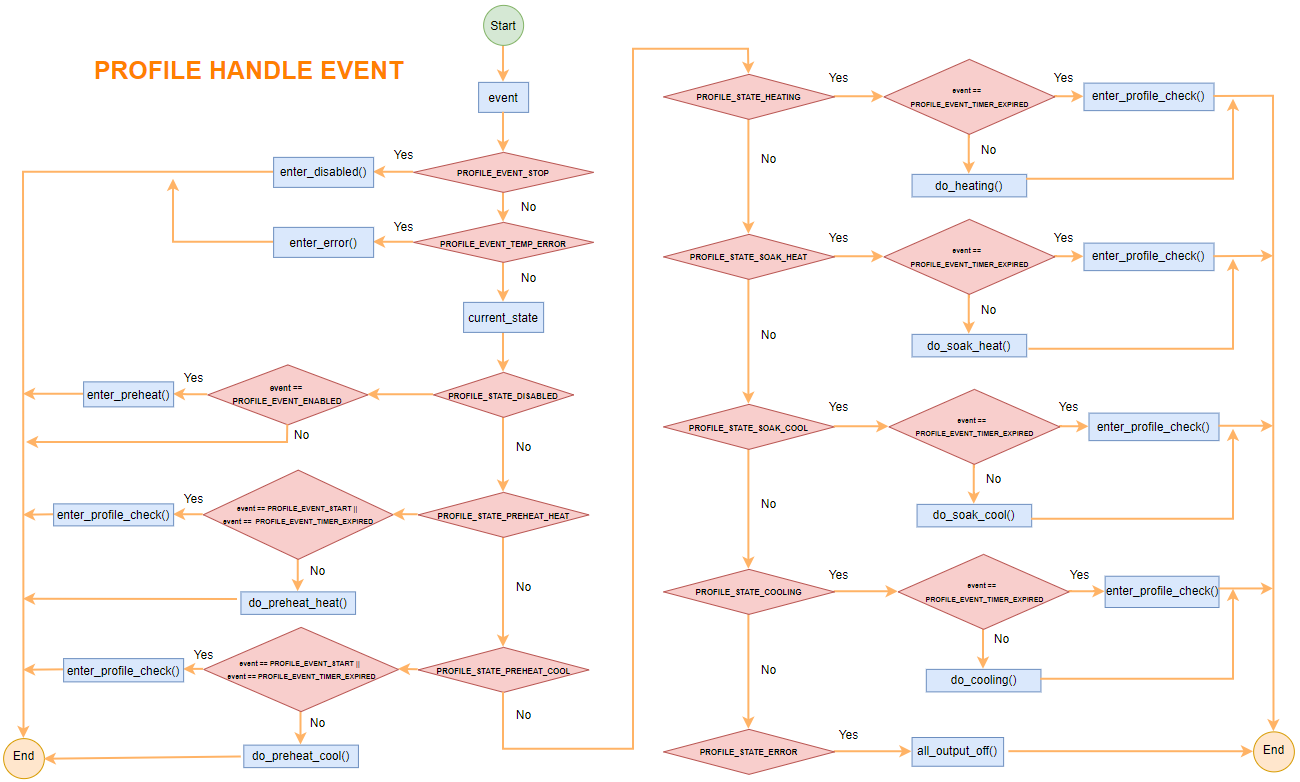
\includegraphics[angle=90,width=0.9\textwidth]
    {picture/firmware/Temperature_Control/profile-handle-event.png}
    \caption{Lưu đồ giải thuật xử lý sự kiện của phần mềm giám sát nhiệt độ}
    \label{fig:lưu-đồ-giải-thuật-xử-lý-sự-kiện-của-phần-mềm-giám-sát-nhiệt-độ}
\end{figure}

\paragraph{Cơ chế chuyển trạng thái và xử lý an toàn}

\begin{itemize}

    \item \textbf{Ưu tiên xử lý sự kiện an toàn}
    
    Hai sự kiện:
    
    \begin{center}
        \texttt{PROFILE\_EVENT\_STOP}
        
        \texttt{PROFILE\_EVENT\_TEMP\_ERROR}
    \end{center}
    
    luôn được kiểm tra đầu tiên trong chu kỳ xử lý.
    
    Khi phát hiện một trong hai sự kiện trên, hệ thống sẽ lập tức gọi:
    
    \begin{itemize}
        \item \texttt{enter\_disabled()}
        \item hoặc \texttt{enter\_error()}
    \end{itemize}
    
    nhằm đưa hệ thống về trạng thái an toàn và bảo vệ phần cứng ngay khi xảy ra sự cố. Sự kiện 

    \item \textbf{Trạng thái nghỉ (\texttt{DISABLE})}
    
    Đây là trạng thái mặc định khi hệ thống khởi động.
    
    Khi nhận sự kiện:
    
    \begin{center}
        \texttt{PROFILE\_EVENT\_ENABLED}
    \end{center}
    
    hệ thống sẽ gọi hàm:
    
    \begin{center}
        \texttt{enter\_preheat()}
    \end{center}
    
    để bắt đầu quá trình chuẩn bị nhiệt độ ban đầu.

    \item \textbf{Giai đoạn PREHEAT}
    
    Trong giai đoạn này, hệ thống liên tục so sánh nhiệt độ thực tế với giá trị đặt:
    
    \begin{center}
        \texttt{temp} $\leftrightarrow$ \texttt{set\_point}
    \end{center}
    
    \begin{itemize}
        \item Nếu nhiệt độ thấp hơn \textit{setpoint}:
        
        Hệ thống chuyển sang trạng thái:
        \texttt{PREHEAT\_HEAT},
        
        đồng thời khởi tạo bộ PID và cấu hình bộ điều khiển cho Heater.
        
        \item Nếu nhiệt độ cao hơn \textit{setpoint}:
        
        Hệ thống chuyển sang trạng thái:
        \texttt{PREHEAT\_COOL},
        
        đồng thời khởi tạo bộ PID và cấu hình điều khiển cho TEC.
    \end{itemize}
    
    Giai đoạn này kết thúc khi hệ thống nhận:
    
    \begin{itemize}
        \item \texttt{PROFILE\_EVENT\_START}
    \end{itemize}
    
    Sau đó, hệ thống gọi:
    
    \begin{center}
        \texttt{enter\_profile\_check()}
    \end{center}
    
    để điều phối các trạng thái vận hành tiếp theo.

    \item \textbf{Trạng thái \texttt{HEATING}/\texttt{COOLING}}
    
    Trong quá trình thay đổi nhiệt độ:
    
    \begin{itemize}
        \item Nếu chưa hết thời gian quy định, hệ thống liên tục thực thi:
        
        \begin{itemize}
            \item \texttt{do\_heating()}
            \item hoặc \texttt{do\_cooling()}
        \end{itemize}
        
        để cập nhật PID và điều chỉnh công suất đầu ra.
        
        \item Khi hết thời gian Ramp:
        
        Hệ thống gọi:
        
        \begin{center}
            \texttt{enter\_profile\_check()}
        \end{center}
        
        để chuyển sang bước tiếp theo trong \textit{Profile}.
    \end{itemize}

    \item \textbf{Trạng thái Soak (\texttt{HOLD\_ON})}
    
    Trong giai đoạn giữ nhiệt, hệ thống thực thi:
    
    \begin{itemize}
        \item \texttt{do\_soak\_heat()}
        \item hoặc \texttt{do\_soak\_cool()}
    \end{itemize}
    
    nhằm duy trì nhiệt độ ổn định quanh giá trị \textit{setpoint}.
    
    Quá trình này tiếp tục cho đến khi nhận được sự kiện:
    
    \begin{center}
        \texttt{PROFILE\_EVENT\_TIMER\_EXPIRED}
    \end{center}


\end{itemize}

Sơ đồ khối của trạng thái HEATING và COOLING:

\begin{figure}[H]
    \centering
    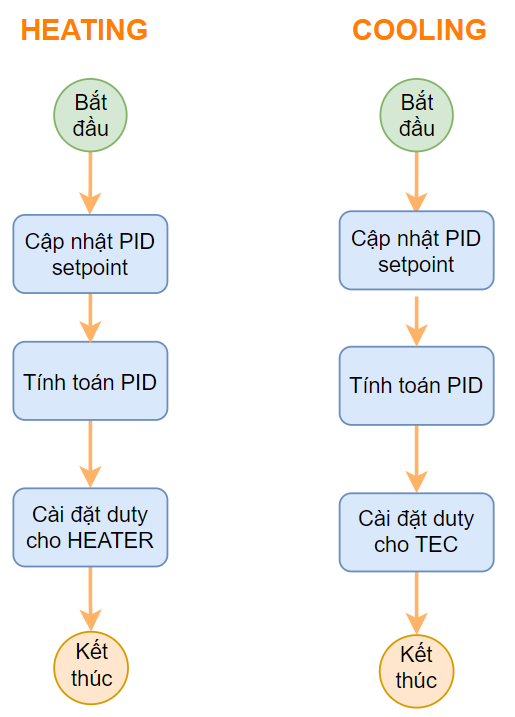
\includegraphics[width=0.6\textwidth]{picture/firmware/Temperature_Control/heating-cooling.png}
    \caption{Sơ đồ khối trạng thái HEATING và COOLING}
    \label{fig:so-do-khoi-heating-cooling}
\end{figure}

Ở trạng thái này, hệ thống cũng sẽ tính toán PID để xuất PWM cho HEATER hoặc TEC nhưng không giống như ở trạng thái \texttt{PREHEAT}, hệ thống không lấy setpoint cố định mà dựa vào nhiệt độ mục tiêu trong thời gian bao lâu để chia thành các setpoint trung gian. Mỗi lần vào hàm điều khiển \texttt{do\_heating()} hoặc \texttt{do\_cooling()} thì sẽ cập nhật setpoint để bộ điều khiển PID so sánh nhiệt độ thực tế và điều khiển duty cycle xuất PWM cho TEC hoặc HEATER.

\begin{figure}[H]
    \centering
    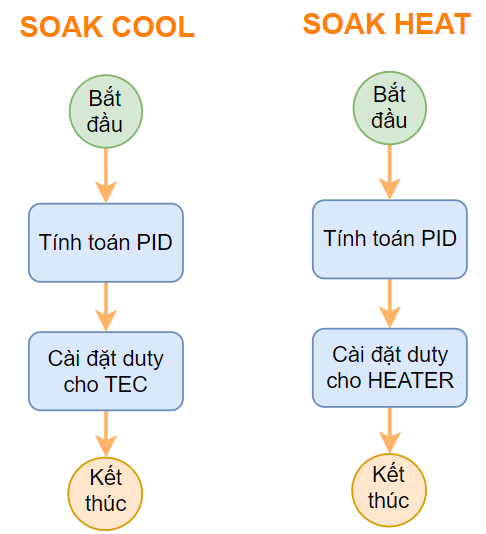
\includegraphics[width=0.6\textwidth]{picture/firmware/Temperature_Control/soak.png}
    \caption{Sơ đồ khối trạng thái SOAK HEAT và SOAK COOL}
    \label{fig:so-do-khoi-soak}
\end{figure}

Ở trạng thái này, PID tiếp tục tính toán PID để duy trì nhiệt độ cho đến khi hết thời gian quy định trong bước của Profile.

\end{itemize}




\newpage